% Created 2024-05-23 木 16:56
% Intended LaTeX compiler: pdflatex
\documentclass[allowframebreaks]{beamer}
\usepackage[utf8]{inputenc}
\usepackage[T1]{fontenc}
\usepackage{graphicx}
\usepackage{longtable}
\usepackage{wrapfig}
\usepackage{rotating}
\usepackage[normalem]{ulem}
\usepackage{amsmath}
\usepackage{amssymb}
\usepackage{capt-of}
\usepackage{hyperref}
\mode<beamer>{\usetheme{Madrid}}
\usetheme{default}
\author{Yuri Guimaraes}
\date{\today}
\title{2024/05/23 Progress Report}
\hypersetup{
 pdfauthor={Yuri Guimaraes},
 pdftitle={2024/05/23 Progress Report},
 pdfkeywords={},
 pdfsubject={},
 pdfcreator={Emacs 27.1 (Org mode 9.7)}, 
 pdflang={English}}
\begin{document}

\maketitle
\begin{frame}{Outline}
\tableofcontents
\end{frame}

\section{Summary}
\label{sec:org4a478bb}
\begin{frame}[label={sec:orgdb8f7f1},fragile]{Summary}
 \begin{block}{Task List}
\begin{enumerate}
\item \sout{Browse \texttt{smartcam} module source code.}
\item \sout{Compile \texttt{smartcam} code.}
\item \sout{Modify \texttt{smartcam} code to use other kernels.}
\item \alert{Write image compression \(\rightarrow\) storage prototype pipeline.}
\end{enumerate}
\end{block}
\end{frame}
\begin{frame}[label={sec:org3ae2dc2},fragile]{Recap (1 / 2)}
 Xilinx's Smart Camera application allows for a

\texttt{MIPI capture} \(\rightarrow\) \texttt{PL processing} \(\rightarrow\) \texttt{RTSP/DP output} pipeline.
\begin{center}
\includegraphics[width=.9\linewidth]{/home/ayyg/.config/emacs/.local/cacheorg/persist/21/02938c-69f5-44dd-af03-c6847df5a023-1aab41956ed65d30ed850321fd664e91.jpg}
\end{center}
\end{frame}
\begin{frame}[label={sec:orgceffcc6}]{Recap (2 / 2)}
This is done via a GStreamer-Video4Linux2 driver.
\begin{center}
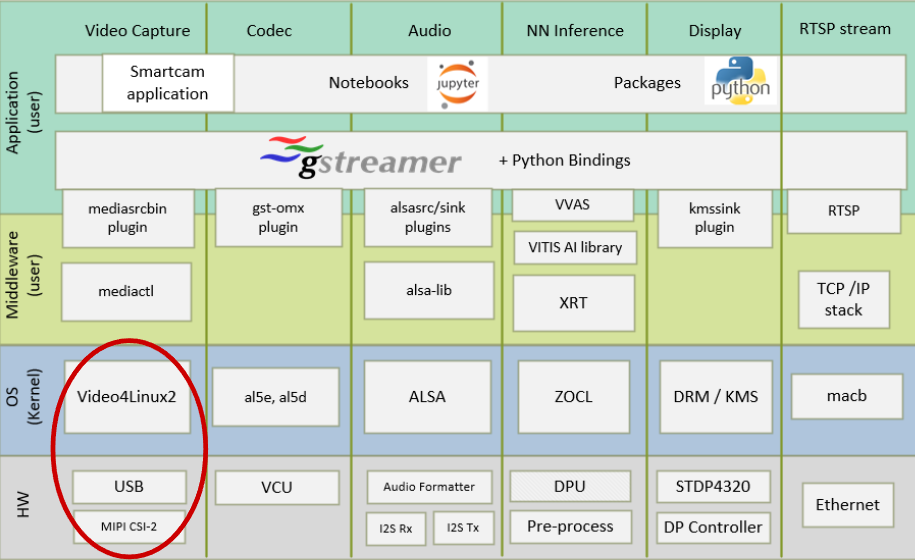
\includegraphics[width=.9\linewidth]{2024-05-23-13-44-56_915x560.png}
\end{center}
\end{frame}
\begin{frame}[label={sec:org444c1eb}]{Objectives}
\begin{block}{Runtime}
\begin{itemize}
\item What is v4l2's role in acquiring the image from DMA?
\item How does GStreamer use v4l2?
\item How does an acceleration kernel run using v4l2/GStreamer?
\end{itemize}
\end{block}
\begin{block}{Building}
\begin{itemize}
\item What does the final software depend on?
\item What does the developer need to have ready in order to build the application?
\begin{itemize}
\item Dependencies?
\end{itemize}
\end{itemize}
\end{block}
\end{frame}
\section{Hardware-Software Architecture}
\label{sec:orgf45aa33}
\begin{frame}[label={sec:org2e6695c},fragile]{MIPI-CSI2 Capture (Hardware)}
 \begin{columns}
\begin{column}{0.4\columnwidth}
\begin{itemize}
\item MIPI source outputs to \texttt{S\_AXI\_HP0\_FPD}.
\item \texttt{NV12} format.
\end{itemize}
\end{column}
\begin{column}{0.6\columnwidth}
\begin{block}{}
\begin{center}
\begin{tabular}{ll}
NV12 & Planar 8-bit YUV 4:2:0\\
YUV420 & \alert{Semi}-planar 8-bit YUV 4:2:0\\
\end{tabular}
\end{center}
\end{block}
\end{column}
\end{columns}
\begin{block}{}
\begin{figure}[htbp]
\centering
\includegraphics[width=.9\linewidth]{/home/ayyg/.config/emacs/.local/cacheorg/persist/0e/2348c2-1ffb-4b6c-ace7-c61a620e45d9-0779a2993e38c2edfd696da45e246478.png}
\caption{MIPI Capture Pipeline}
\end{figure}
\end{block}
\end{frame}
\begin{frame}[label={sec:org0bd9b57},fragile]{MIPI-CSI2 Capture (Software) (1 / 2)}
 \begin{columns}
\begin{column}{0.3\columnwidth}
\begin{itemize}
\item Source accessible via \texttt{v4l2}

\(\rightarrow\) \texttt{/dev/media*}

\(\rightarrow\) \texttt{/dev/video*}

\ldots{}

\(\rightarrow\) \texttt{v4l2src}

\(\rightarrow\) \texttt{mediasrc}
\end{itemize}
\end{column}
\begin{column}{0.7\columnwidth}
\begin{figure}[htbp]
\centering
\includegraphics[height=0.7\textheight]{/home/ayyg/.config/emacs/.local/cacheorg/persist/b1/ed6031-6449-4af6-8d50-b1b6cfa73480-aef2fb32d26d71130fa5a196c313741a.png}
\caption{Video Capture Diagram}
\end{figure}
\end{column}
\end{columns}
\end{frame}
\begin{frame}[label={sec:orgeb6a7fe}]{MIPI-CSI2 Capture (Software) (2 / 2)}
\begin{figure}[htbp]
\centering
\includegraphics[width=.9\linewidth]{/home/ayyg/.config/emacs/.local/cacheorg/persist/3c/d00996-a607-45af-b32f-5c676195e614-183c7e3610f5656b755e98078cc0ea1d.png}
\caption{GStreamer Pipeline}
\end{figure}
\end{frame}
\begin{frame}[label={sec:orgfce1bcf},fragile]{Acceleration}
 Acceleration on the new stack is based on HLS kernels. For vision, there is \texttt{VVAS}.
The Smart Camera application uses \texttt{VVAS} with \texttt{GStreamer}.
\begin{block}{VVAS}
\href{https://www.xilinx.com/products/design-tools/vitis/vvas.html}{Vitis Video Analytics SDK} is Xilinx's software stack for building video processing applications.
\end{block}
\begin{block}{Plugin Structure}
Use \alert{GStreamer} plugins for creating computer vision pipelines.
\end{block}
\end{frame}
\section{GStreamer}
\label{sec:orgec1320b}
\begin{frame}[label={sec:org4ab2d90}]{GStreamer}
\begin{quote}
GStreamer is a pipeline-based multimedia framework linking various media processing systems to create workflows.
\end{quote}
\begin{figure}[htbp]
\centering
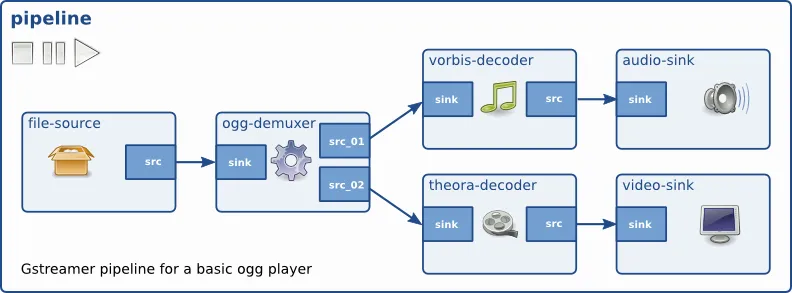
\includegraphics[width=.9\linewidth]{gst.png}
\caption{Example of a GStreamer pipeline.}
\end{figure}
\end{frame}
\begin{frame}[label={sec:org8bff8dc},fragile]{GStreamer Basics}
 \begin{block}{Elements}
Objects derived from \texttt{GstElement}. Examples:
\begin{itemize}
\item \texttt{source} element: provides data
\item \texttt{filter} element: acts on incoming data
\end{itemize}
\end{block}
\begin{block}{Pads}
Objects derived from \texttt{GstPad}. They are the ``ports'' that intermediate data between elements.
\begin{itemize}
\item \emph{Source} pad: data flows outward
\item \emph{Sink} pad: data flows inward
\end{itemize}
\end{block}
\begin{block}{Buffers}
\begin{itemize}
\item \texttt{GstMiniObject}, \texttt{GstBuffer}, \texttt{GstEvent}\ldots{}
\end{itemize}
\end{block}
\end{frame}
\begin{frame}[label={sec:orgf69175f},fragile]{GStreamer Plugins}
 \begin{itemize}
\item Enables plug-and-play functionality with GStreamer.
\item Elements must be wrapped into a plugin before being used.
\end{itemize}
\begin{block}{What is a plugin?}
Essentially, it is a block of loadable code (a shared object/dynamically linked library).
\end{block}
\begin{block}{What is the structure of a plugin?}
\url{https://gitlab.freedesktop.org/gstreamer/gst-template.git}
\begin{itemize}
\item The above serves as good reference.
\item The compiled code generates a \texttt{libgstplugin.so}, which can be loaded by \texttt{gst-launch-1.0} by simply specifying the path in \texttt{GST\_PLUGIN\_PATH}.
\end{itemize}
\end{block}
\end{frame}
\begin{frame}[label={sec:org6fffc8d}]{VVAS}
\begin{itemize}
\item Collection, as well as an API for creating acceleration kernels for usage with GStreamer.
\end{itemize}
\begin{figure}[htbp]
\centering
\includegraphics[height=0.6\textheight]{/home/ayyg/.config/emacs/.local/cacheorg/persist/1c/91e839-5d71-4fb2-9898-3d9aeb2cd569-9287f86b5159ddd00f3fa5620942ae7f.png}
\caption{How VVAS relates to GStreamer}
\end{figure}
\end{frame}
\begin{frame}[label={sec:org0824bf6},fragile]{VVAS Usage in GStreamer (1 / 2)}
 API usage:
\begin{enumerate}
\item Plugin Initialization (\texttt{xlnx\_kernel\_init})
\item Kernel Start (\texttt{xlnx\_kernel\_start})
\item Waiting for the kernel to finish (\texttt{vvas\_kernel\_done})
\item Denitilizating the plugin (\texttt{xlnx\_kernel\_deinit})
\end{enumerate}
\end{frame}
\begin{frame}[label={sec:org1dbcf77},fragile]{VVAS Usage in GStreamer (2 / 2)}
 \begin{columns}
\begin{column}{0.4\columnwidth}
\href{https://xilinx.github.io/VVAS/main/build/html/docs/common/gstreamer\_plugins/plugin\_vvas\_xfilter.html}{\texttt{vvas\_xfilter}}:\\
\begin{block}{JSON config}
Contains information regarding:
\begin{itemize}
\item \texttt{xclbin} location
\item \texttt{vvas-library-repo}
\item \texttt{element-mode} (passthrough, inplace, transform)
\end{itemize}
\end{block}
\begin{block}{\texttt{xclbin}}
Used to program the FPGA.
\end{block}
\end{column}
\begin{column}{0.6\columnwidth}
\begin{figure}[htbp]
\centering
\includegraphics[height=0.6\textheight]{/home/ayyg/.config/emacs/.local/cacheorg/persist/23/96419e-e218-4252-9c5a-d2ba65429999-17df4c2226593e47680dff5980db1657.png}
\caption{\texttt{xfilter} usage.}
\end{figure}
\end{column}
\end{columns}
\end{frame}
\section{Source Code Analysis}
\label{sec:orge9fb6fc}
\begin{frame}[label={sec:org3fdde4d},fragile]{Smart Camera --- Folder Structure}
 \begin{itemize}
\item \href{https://github.com/Xilinx/smartcam/tree/2021.1}{\texttt{smartcam}}: Contains the base smartcam application.
It is built and used with Docker.
\end{itemize}
\begin{columns}
\begin{column}{0.4\columnwidth}
\begin{center}
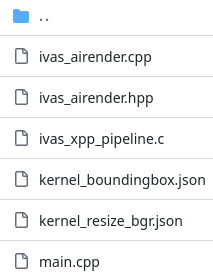
\includegraphics[width=.9\linewidth]{smartcam_repo.png}
\end{center}
\end{column}
\begin{column}{0.6\columnwidth}
\begin{block}{\texttt{smartcam/src}}
\texttt{ivas\_airender}: aadasda\\
\texttt{ivas\_xpp\_pipeline}: aadasda\\
\texttt{main}: Contains the GStreamer pipelines that run everything.
\end{block}
\end{column}
\end{columns}
\end{frame}
\begin{frame}[label={sec:org66433af},fragile]{VVAS Usage in \texttt{smartcam}}
 \href{https://xilinx.github.io/VVAS/main/build/html/docs/common/gstreamer\_plugins/plugin\_vvas\_xfilter.html}{\texttt{vvas\_xfilter}}: Plugin to act directly on data with the specified kernel.
\begin{center}
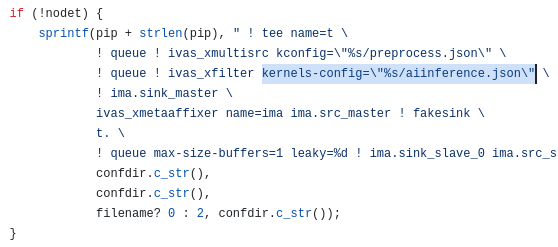
\includegraphics[height=0.6\textheight]{xfilter.png}
\end{center}
\end{frame}
\begin{frame}[label={sec:org40f721d},fragile]{VVAS Example --- Edge Filter with \texttt{filter2d} (1 / 3)}
 \begin{itemize}
\item \alert{\href{https://github.com/Xilinx/vck190-base-trd/tree/2022.1/overlays/filter2d/kernels/filter2d\_pl/}{\texttt{filter2d} source code}}
\end{itemize}
\begin{block}{Makefile}
\begin{center}
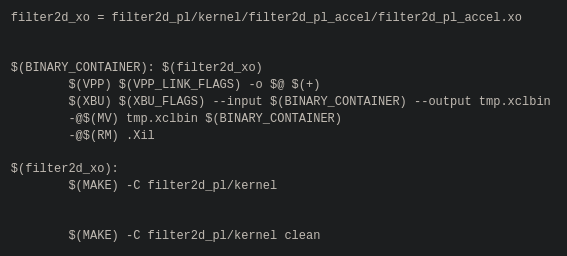
\includegraphics[height=0.6\textheight]{filter2d_makefile.png}
\end{center}
\end{block}
\end{frame}
\begin{frame}[label={sec:org8f22d8b},fragile]{VVAS Example --- Edge Filter with \texttt{filter2d} (2 / 3)}
 \begin{itemize}
\item \alert{\href{https://github.com/Xilinx/vck190-base-trd/tree/2022.1/overlays/filter2d/kernels/filter2d\_pl/}{\texttt{filter2d} source code}}
\end{itemize}
\begin{block}{PS Connectivity}
\begin{center}
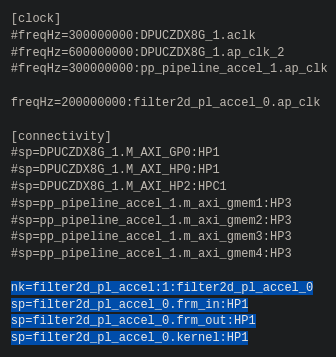
\includegraphics[height=0.6\textheight]{filter2d_connection.png}
\end{center}
\end{block}
\end{frame}
\begin{frame}[label={sec:orgddff004},fragile]{VVAS Example --- Edge Filter with \texttt{filter2d} (3 / 3)}
 \begin{exampleblock}{Launching GStreamer with filter2d kernel}\label{sec:orgf21fe22}
\begin{verbatim}
gst-launch-1.0 v4l2src \
  device=/dev/video0 io-mode=mmap !\
  "video/x-raw, width=640, height=480" !\
  videoconvert !\
  "video/x-raw, width=640, height=480,
   format=YUY2, framerate=30/1" !\
  vvas_xfilter kernels-config=/tmp/kernel_xfilter2d_pl.json\
  dynamic-config='{ "filter_preset" : "edge" }' !\
  perf ! kmssink plane-id=39 fullscreen-overlay=true -v
\end{verbatim}
\end{exampleblock}
\end{frame}
\begin{frame}[label={sec:orgfc59722}]{VVAS Example --- Results of the Edge Filter}
\begin{center}

\includegraphics[width=.9\linewidth]{edges.jpg}
\end{center}
\end{frame}
\section{Conclusion}
\label{sec:org66f1420}
\begin{frame}[label={sec:org0d96224}]{Conclusion}
\begin{itemize}
\item Got smartcamera to work on Docker inside the KV260
\begin{itemize}
\item It also worked with a modified kernel
\end{itemize}
\item Next: \alert{Write image compression \(\rightarrow\) storage prototype pipeline?}
\item I'm also working on making the build process for these packages simple.
\end{itemize}
\end{frame}
\begin{frame}[label={sec:org9a9560d}]{Appendix}
\begin{block}{AIBox-ReID}
Xilinx demo for 4k IP cameras as inputs on the KV260.
\begin{center}
\includegraphics[width=.9\linewidth]{/home/ayyg/.config/emacs/.local/cacheorg/persist/60/643beb-9f3c-4873-b7c3-529b34d8be7b-f368911fa4a3a0fec8c7d84c885417ae.jpg}
\end{center}
\end{block}
\end{frame}
\begin{frame}[label={sec:org35d1c1e}]{Appendix}
\begin{block}{AI Box Distributed ReID}
Distributed demo.
\begin{center}
\includegraphics[width=.9\linewidth]{/home/ayyg/.config/emacs/.local/cacheorg/persist/66/a76632-69f6-452b-8f31-7bf16d452162-ed2e41a716b3ebbdad9a6ba6a0eba84e.png}
\end{center}
\end{block}
\end{frame}
\end{document}
